\chapter{\MakeUppercase{Шагающие роботы}}

\section{Задачи работы}

В рамках работы рассматривается разработка шагающего четырехногого робота, с упором на проблему разработки конечностей, подбора электроприводов и их управления. Сравниваться будут два типа электроприводов: заводские микро-сервоприводы с редуктором и бесколлекторные синхронные двигатели (BLDC). 

Требуется:
\begin{itemize}
    \item Рассчитать худший (по нагрузке) статический случай для конечностей 4-х ногого робота.
    \item Подобрать два электропривода удовлетворяющих по крутящему моменту. Для двух типов электроприводов разработать модель конечностей.
    \item Собрать физическую модель конечностей двух типов.
    \item Сравнить управляемость и механические характеристики конечностей двух типов.
    \item Применить самую удачную конструкцию конечностей при сборке робота.
    \item Запрограммировать управление робота.
\end{itemize}

\section{Актуальность работы}

Задача разработки конечностей для шагающих роботов настолько же важная, как и задача навигации роботов. Сегодня она актуальна, как никогда ранее. Всё в большей степени людей стараются заменять шагающими роботами для работ вроде общего тех. осмотра помещений, исследования местности вдали от дорог и цивилизации, помощи в устранении последствий катастроф. Открытость методик, исходных кодов и готовых рассчитанных моделей приведет к массовой разработке шагающих роботов не только крупными предприятиями, но и мелкими разработчиками.

\section{Анализ}

Для поставленных ранее задач можно сформировать последовательность действий, которые приведут к их решению.

\subsection{Рассчёт худшего статического случая}

«Худшим» случаем называется такой, при котором одному или нескольким приводам нужно приложить максимальный момент для поворота звена конечности в нужную сторону.

Для того чтобы определить худший случай, нужно вообще определиться с кинематикой конечности. Оптимальной кинематикой можно считать конечность с 3 степенями свободы:

\begin{figure}[ht]
    \centering
    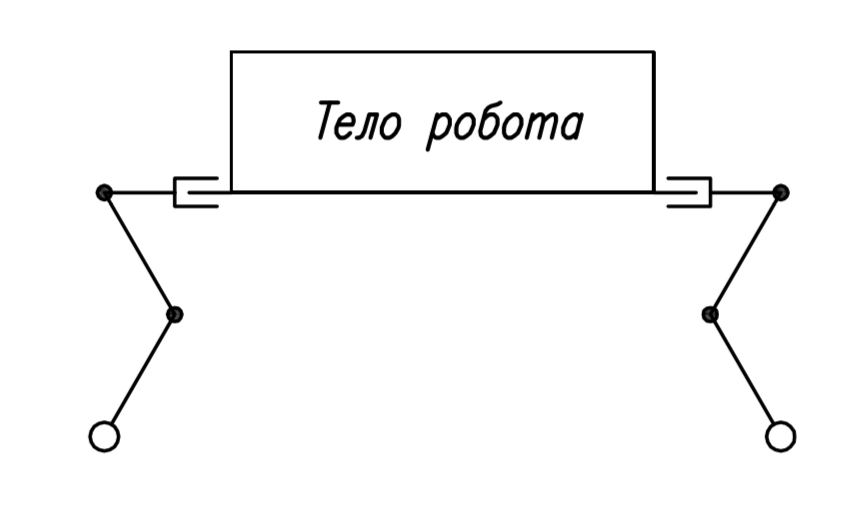
\includegraphics[scale=0.7]{kin1.png}
    \caption{Кинематика 4-х ногого робота, вид сбоку}
\end{figure}

Худшим случаем считается случай, в котором робот лежит на «животе» с выпрямленной конечностью. Чтобы подогнуть под себя конечность, нужно будет преодолеть момент $M_{худш}$ с учетом массы тела робота $m$.

\begin{figure}[ht]
    \centering
    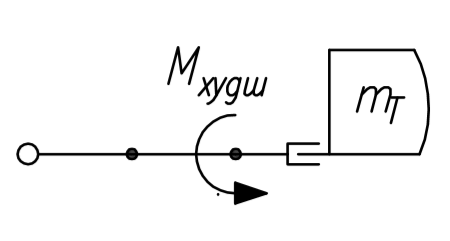
\includegraphics[scale=1]{kin2.png}
    \caption{Кинематика 4-х ногого робота, вид сбоку (худший случай)}
\end{figure}

При расчёте в первом приближении можно пренебречь трением и весами звеньев. Также можно учесть, что нагрузка, создаваемая массой тела робота будет распределена равномерно по всем 4-м ногам. Это значит что на одну ногу будет приходится лишь $\frac{1}{4}m$ тела робота.

Также, в первом приближении допустим, что тело робота может достигать 2-х килограмм. Большая часть веса придется на каркас конструкции, собранный из пластика. Меньшая часть веса придется на аккумулятор. Еще более маленькая часть придется на проводку и крепежи. Самыми легкими составляющими конструкции окажутся электронные компоненты.

При таком расчете можно считать что каждой ноге надо будет «поднять» около 0.25 кг веса. Тогда в худшем случае, приложенный момент вычисляется просто:
$$ M_{худш}=(l_{1}+l_{2}) m g, $$
\noindent здесь $l_1$ и $l_2$ - длины звеньев.

Мы можем подобрать длины звеньев таким образом, чтобы они обеспечивали достаточную для задач ходьбы рабочую область и одновременно наименьший требуемый момент. Однако сначала нам нужно будет измерить реальные моменты на подобранных электроприводах.

\subsection{Подбор электроприводов}

Исходя из ожидаемых моментов и скоростей были выбраны два вида электроприводов:

\begin{itemize}
    \item Заводской сервопривод DSSERVO RDS3225
    \item BLDC-мотор DYS BGM5208-200-12
\end{itemize}

Использовать паспортные данные двигателей для расчётов нельзя, нужно измерить их реальный момент вращения. Для измерения крутящих моментов были разработаны стенды, принцип действия которых можно описать следующей схемой:

\begin{figure}[ht]
    \centering
    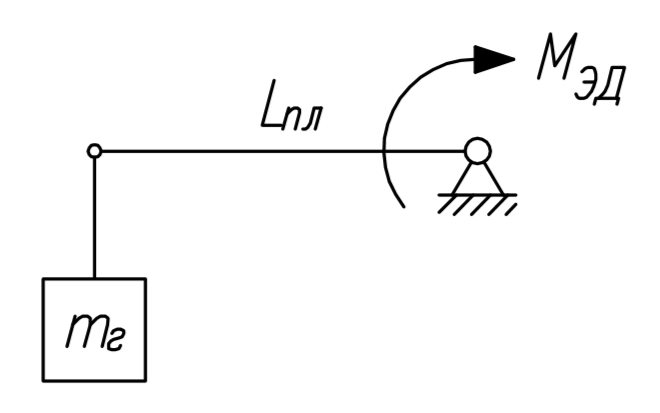
\includegraphics[scale=0.7]{kin3.png}
    \caption{Кинематика стенда для измерения крутящего момента}
\end{figure}

На изображении $ m_г $ - масса груза, которая нам известна, и которую мы можем менять. $ L_{пл} $ - длина плеча, также известная нам. Из приведенных величин можно легко найти экспериментально значение момента $ M_ {ЭД} $.

Чертеж стенда для BLDC двигателя:

\begin{figure}[ht]
    \centering
    % левая картинка
    \begin{subfigure}[b]{0.45\textwidth}    
        \centering
        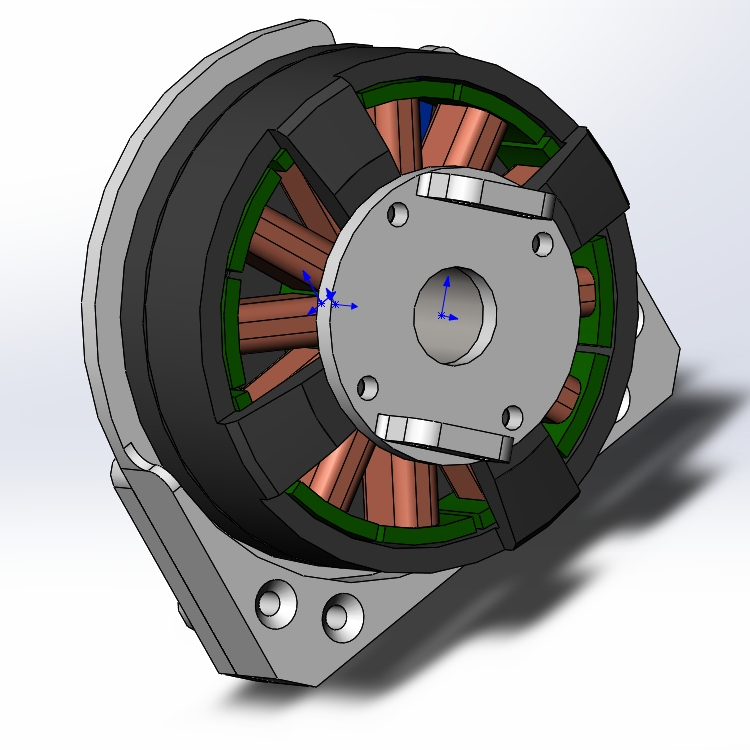
\includegraphics[scale=0.25]{drw1.png}
        \caption{}
    \end{subfigure}
    % правая картинка  
    \begin{subfigure}[b]{0.45\textwidth}
        \centering
        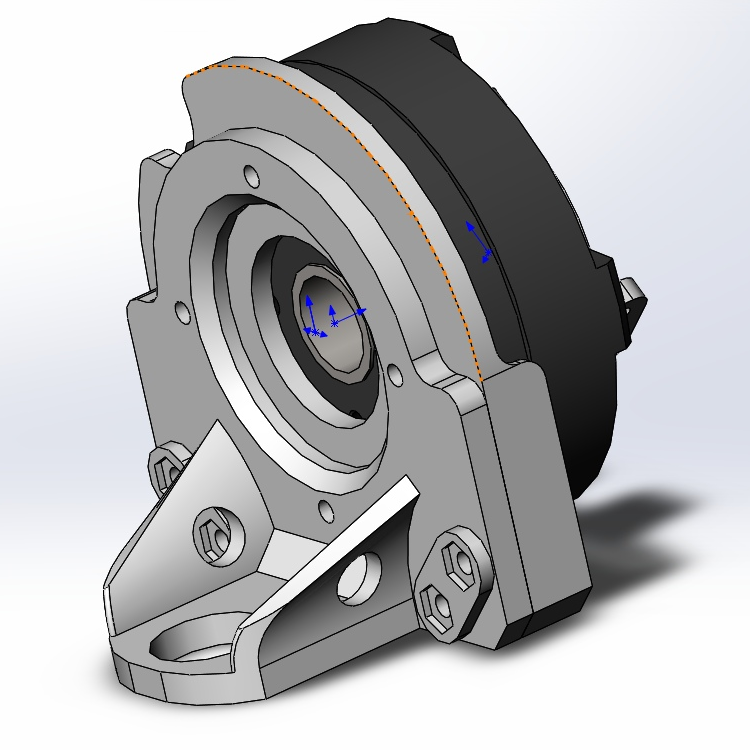
\includegraphics[scale=0.25]{drw2.png}
        \caption{}
    \end{subfigure}
     
    \caption{(a) Стенд для измерения крутяжего момента BLDC мотора, вид спереди; (б) Тот же стенд, вид сзади.}
    \label{fig_bldc_test_drawings}
\end{figure}